\documentclass{beamer}
\usetheme{Madrid}

\usepackage[utf8]{inputenc}
\usepackage{polski}
\usepackage{graphicx}
\usepackage[export]{adjustbox}

\graphicspath{ {images/} }
 
\title[Głosowanie elektroniczne]{Dlaczego jeszcze nie głosujemy elektronicznie?}
\author{Jakub Zadrożny}
\institute[II UWr]{
	Instytut Informatyki UWr.
}
\date{3 stycznia 2017}
 
\begin{document}
 
\frame{\titlepage}
 
\begin{frame}
\frametitle{Czy to w ogóle potrzebne?}
\pause
\begin{itemize}
\item
Informatyka jest wszędzie: urzędy, szkoły, uniwersytety, przedsiębiorstwa, maszyny. \pause
\item
Tylko nie na wyborach (przynajmniej nie wszędzie). \pause
\item 
Co moglibyśmy zyskać? \pause
\begin{itemize}
\item Przyspieszyć liczenie wyników. \pause
\item Wyeliminować ludzkie błędy (przecież komputery się nie mylą). \pause
\item Ułatwić głosowanie osobom niepełnosprawnym. \pause
\item Zmniejszyć koszty (np. pozbywając się ogromnych ilości papierowych głosów). \pause
\item Poprawić bezpieczeństwo?
\end{itemize}
\end{itemize}
\end{frame}

\begin{frame}
\frametitle{Podział}
Głosowanie elektroniczne można podzielić na dwie kategorie: \pause
\begin{itemize}
\item e-voting - głosowanie odbywa się w lokalu wyborczym, \pause
\item i-voting - głosowanie odbywa się przez internet.
\end{itemize}
\end{frame}

\begin{frame}
\frametitle{Lever machines}
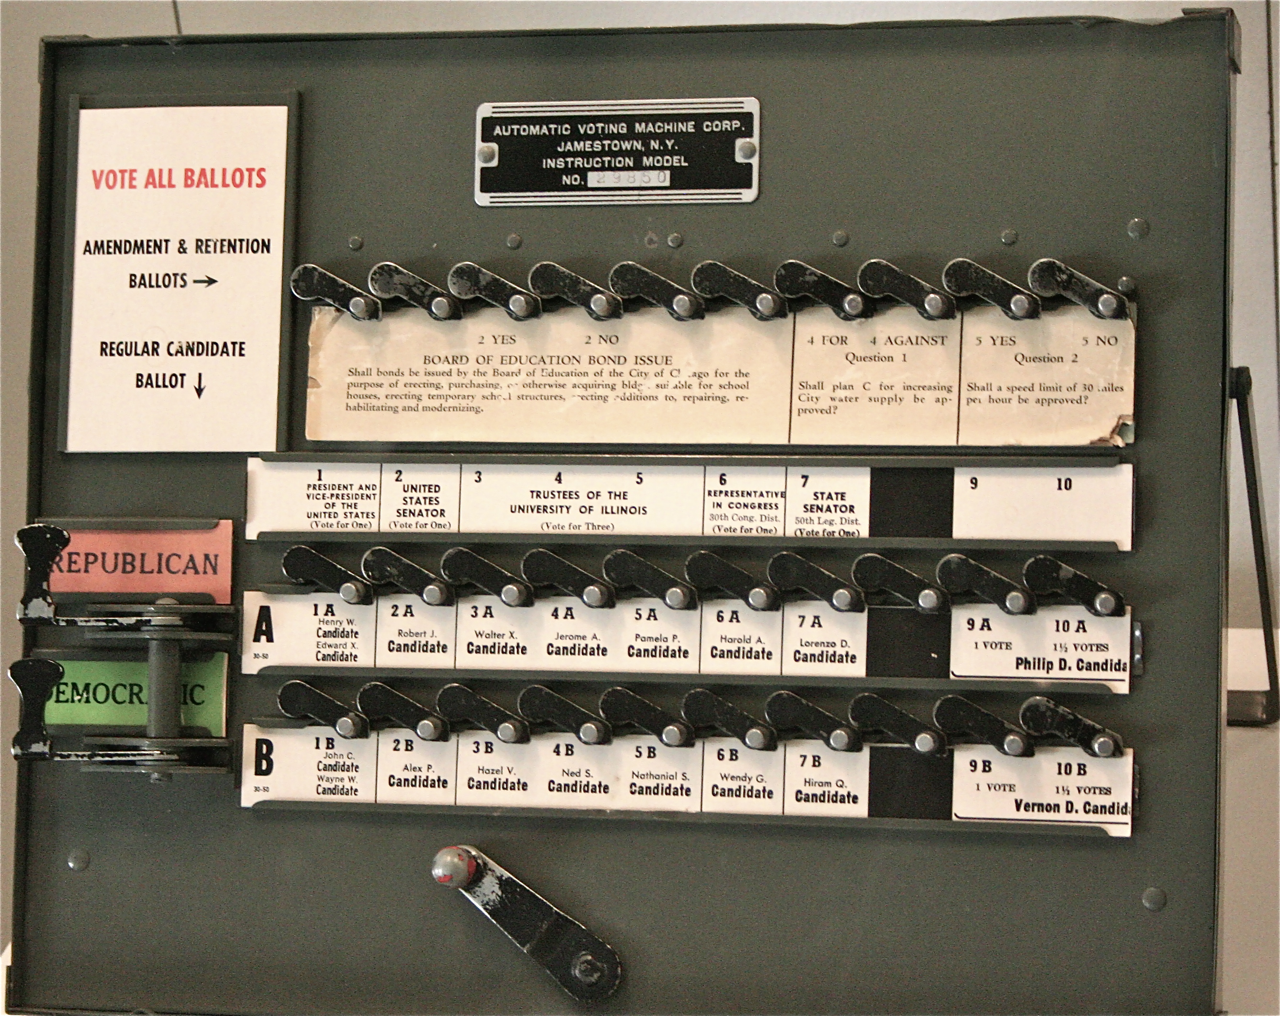
\includegraphics[height=0.65\paperheight, center]{lever} \\ \pause
Zostały wprowadzone do użytku pod koniec XIX wieku i szybko zyskały popularność. \pause W 1960 ponad połowa głosów w USA była rejestrowana przy ich użyciu. \pause Ze Stanów wycofano je dopiero w 2010.
\end{frame}

\begin{frame}
\frametitle{Skanowanie optyczne}
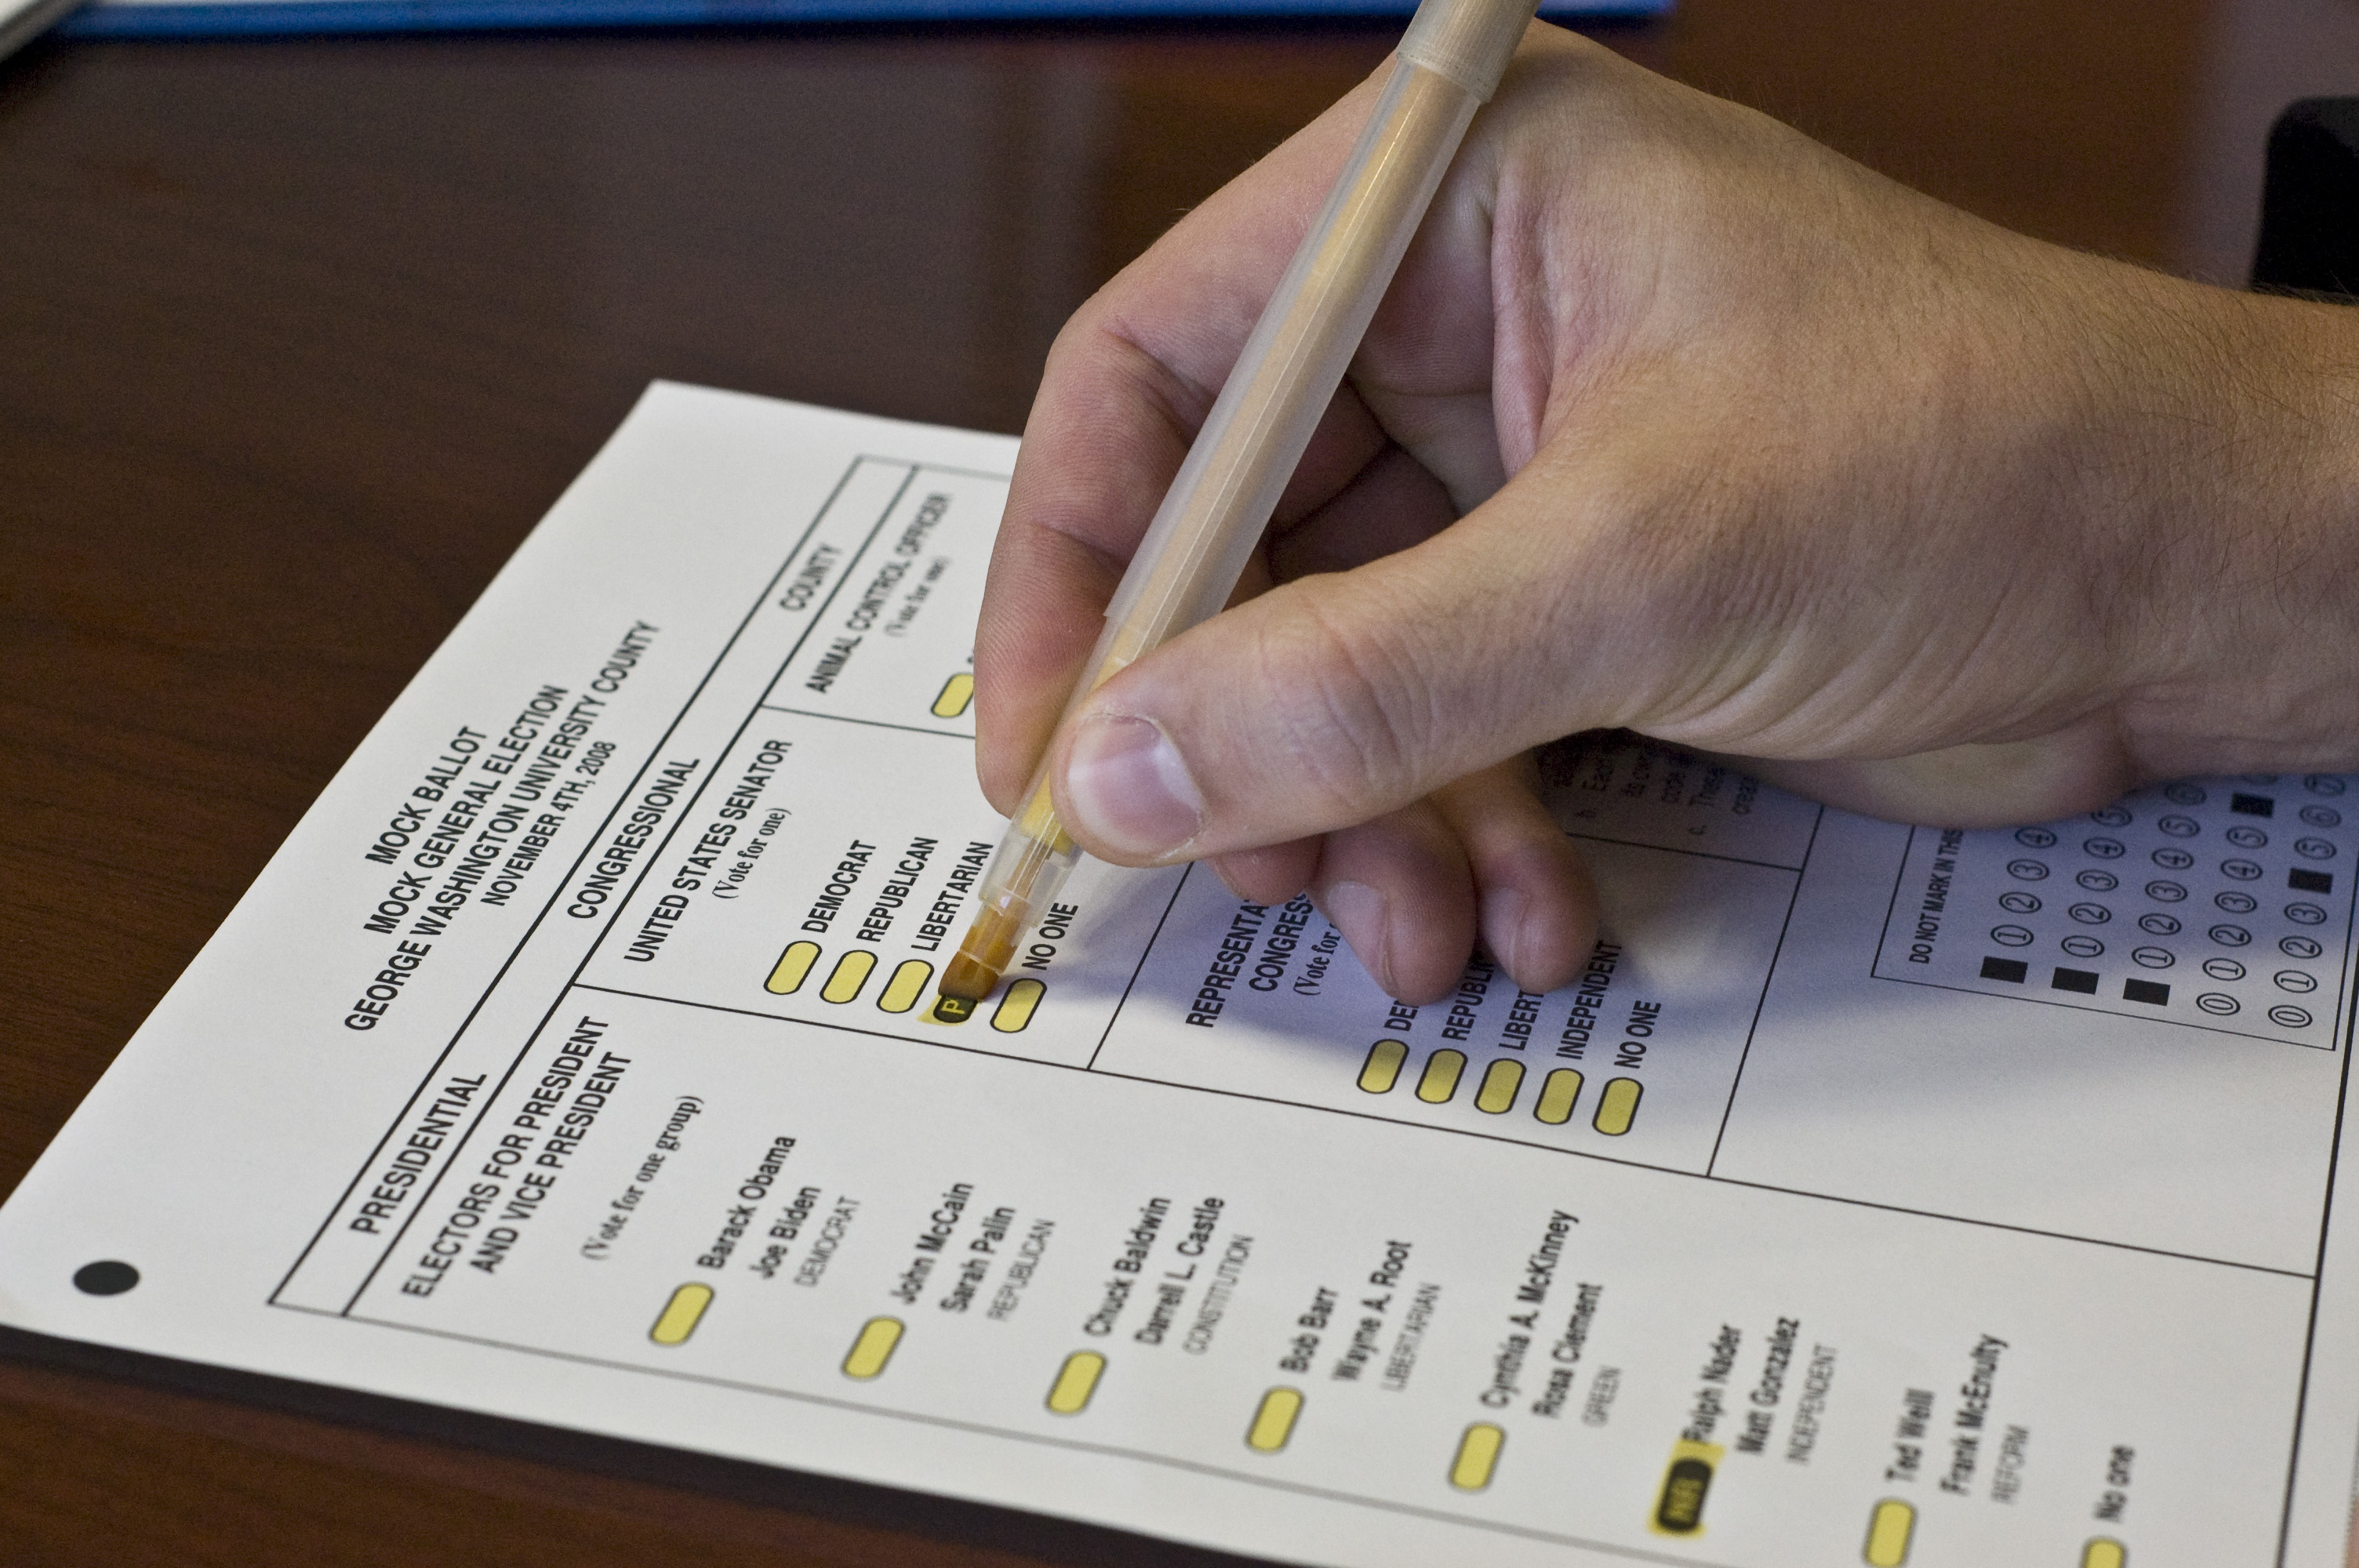
\includegraphics[height=0.7\paperheight, center]{optical} \\ \pause
W USA stosowane nieprzerwanie od 1964. \pause W 1996 wykorzystano je przy zliczaniu 60\% głosów w Stanach.
\end{frame}

\begin{frame}
\frametitle{Direct Recording Electronics}
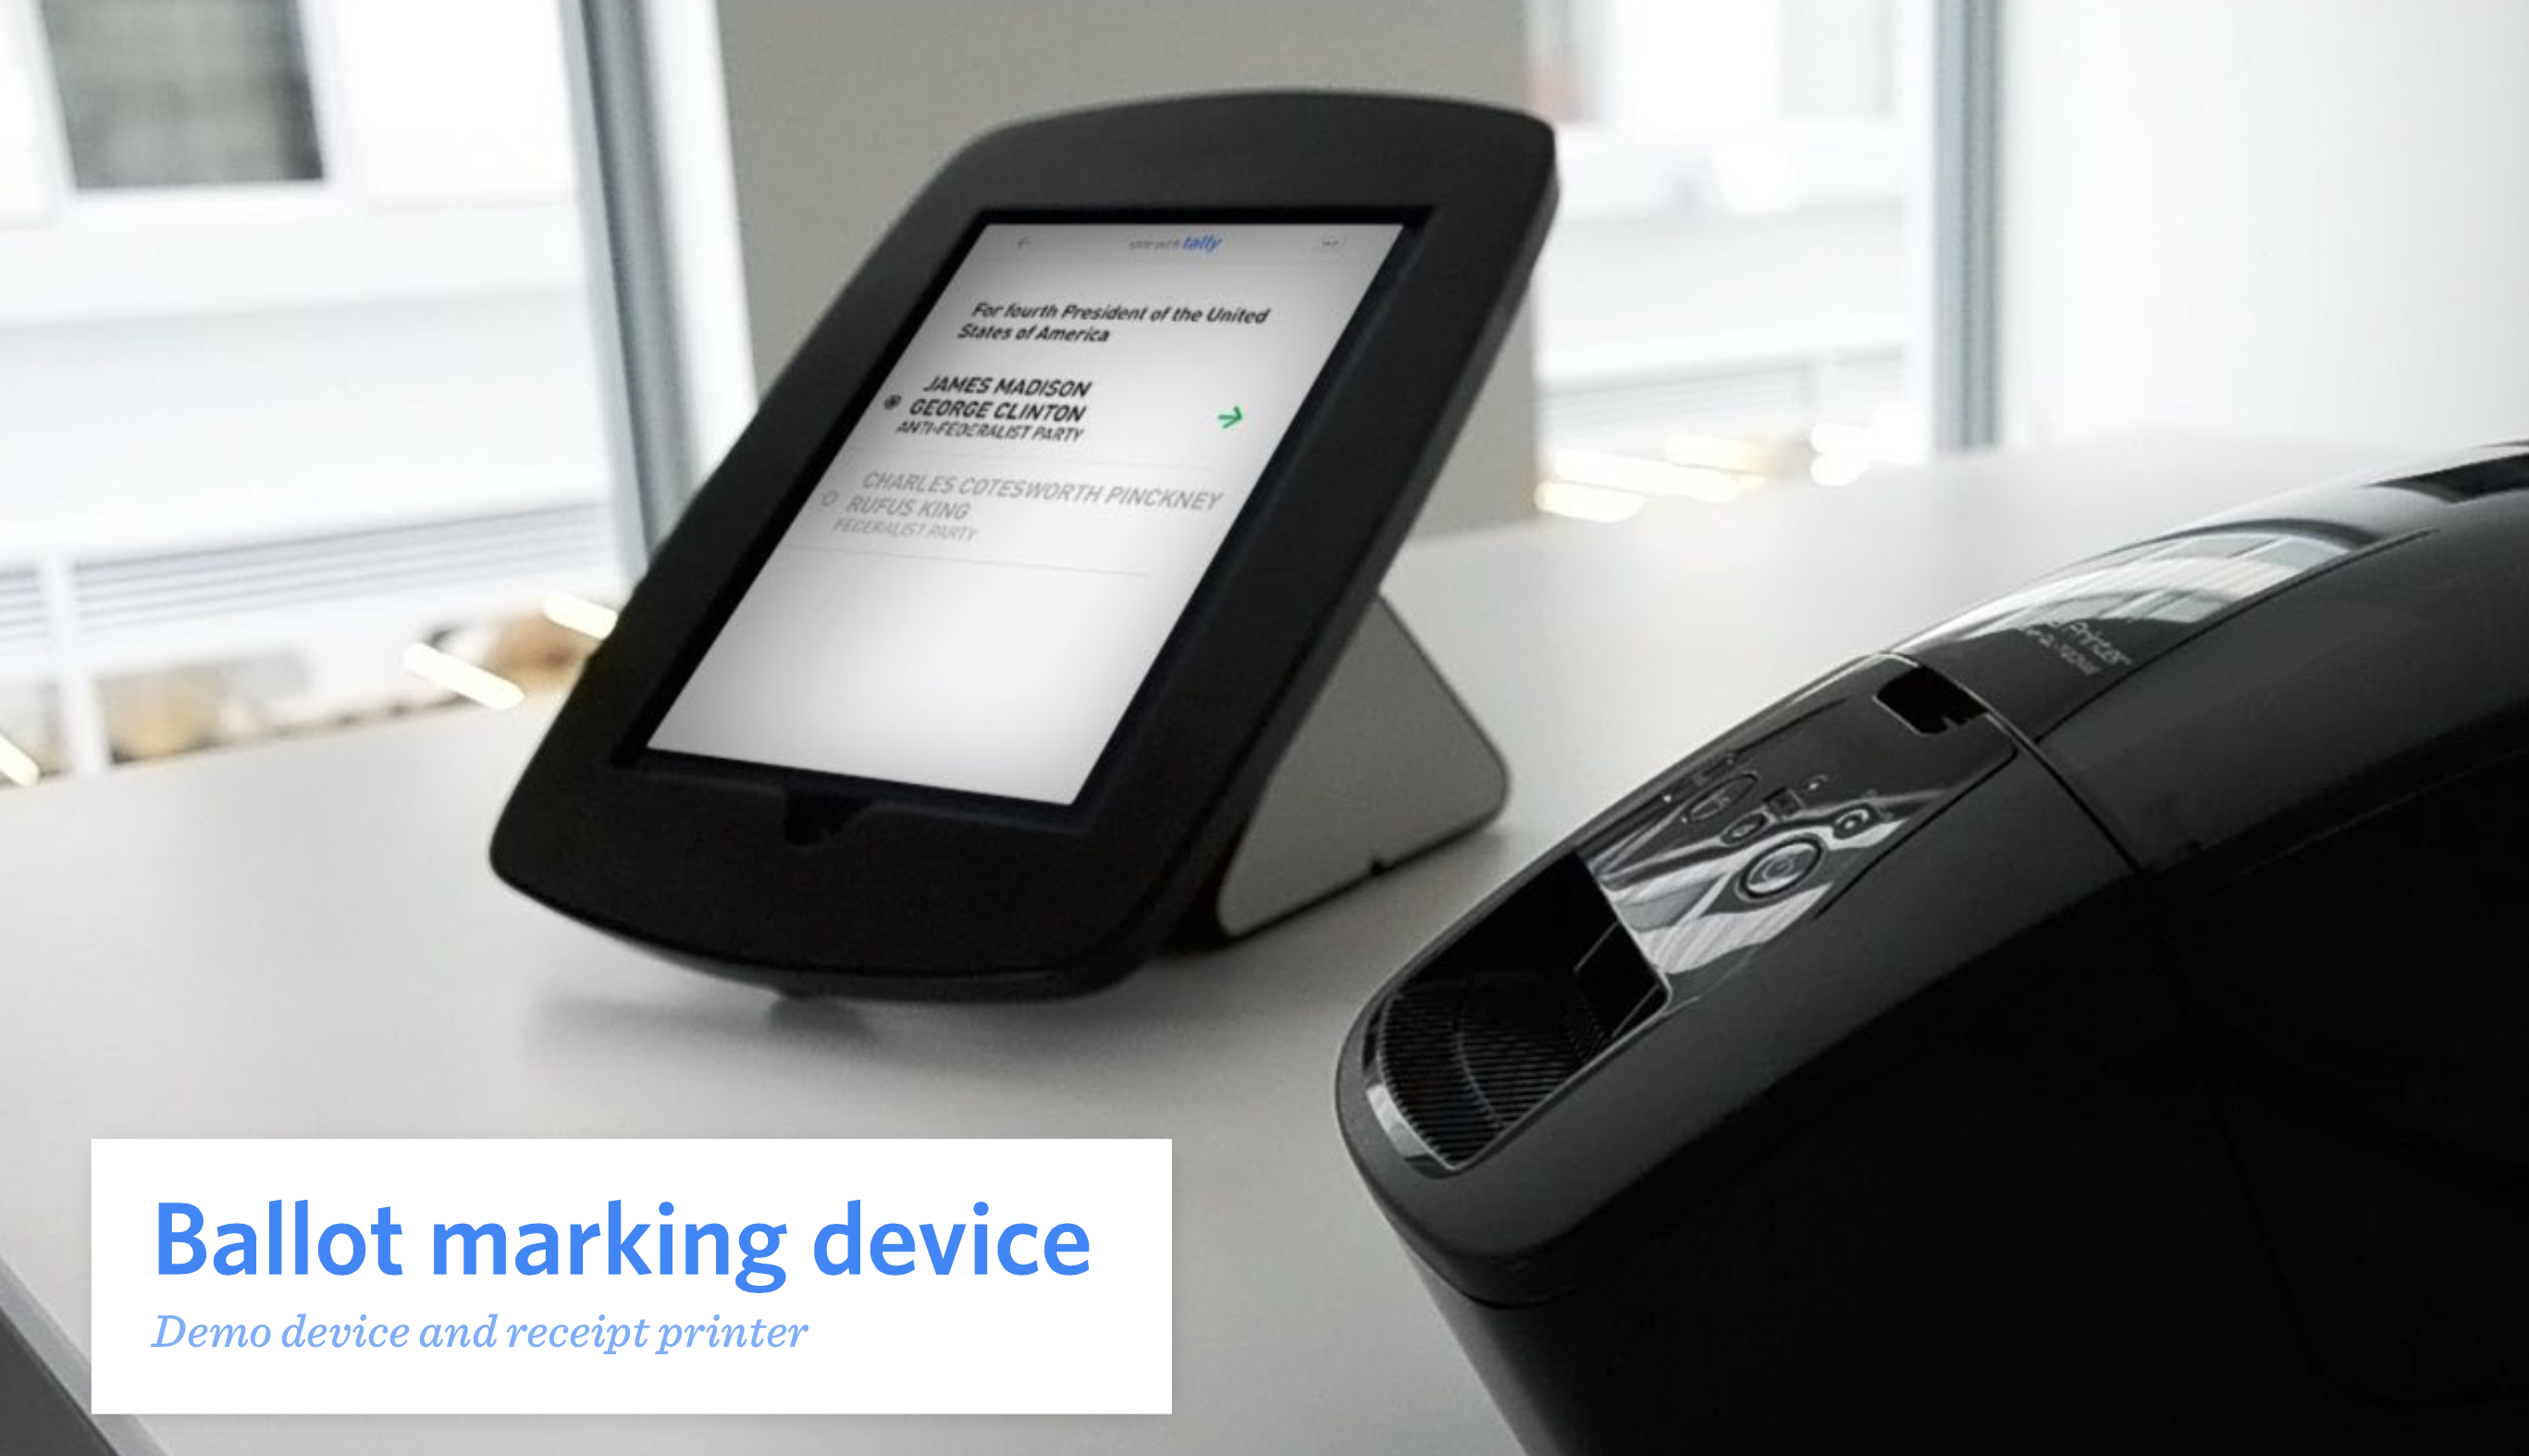
\includegraphics[height=0.65\paperheight, center]{dre} \\ \pause
Na dużą skalę wykorzystywane m.in. w Brazylii (od 1996), Indiach (od 2003) oraz USA. \pause Próbowano wprowadzić je w Holandii oraz Kazachstanie, ale na skutek protestów społecznych pomysł porzucono.
\end{frame}

\begin{frame}
\frametitle{Poczta elektroniczna i fax}
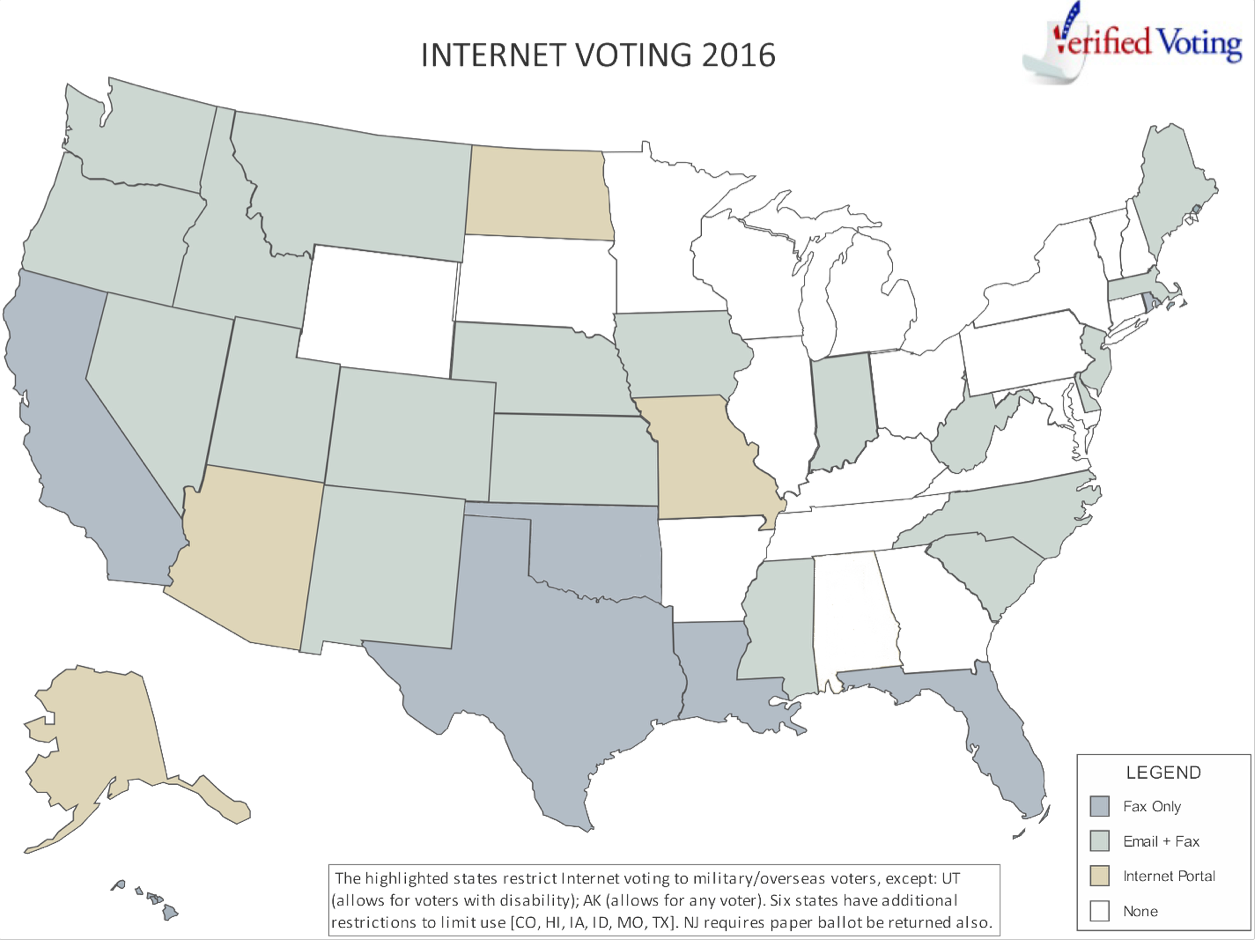
\includegraphics[height=0.65\paperheight, center]{email} \\ 
Ta metoda dopuszczana jest m.in. w USA, Francji i Szwajcarii dla żołnierzy przebywających poza granicami kraju oraz ekspatriantów.
\end{frame}

\begin{frame}
\frametitle{Aplikacje webowe}
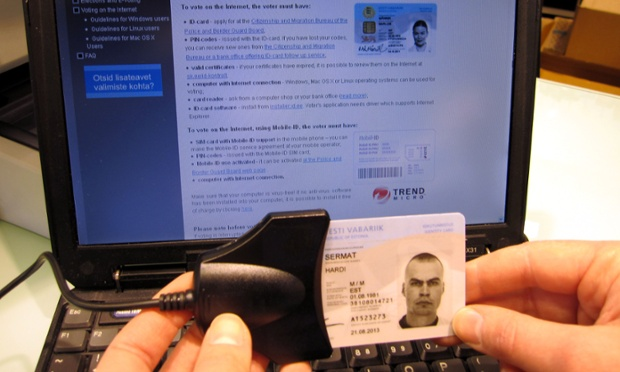
\includegraphics[height=0.6\paperheight, center]{estonia} \\ \pause
Wdrożenia takiego systemu na dużą skalę podjęła się tylko Estonia. \pause Po raz pierwszy przetestowano rozwiązanie w 2005. Wtedy głos przez internet oddało tylko 2\% obywateli. \pause W 2014 i 2015 było to już ponad 30\%.
\end{frame}

\begin{frame}
\frametitle{Udokumentowane ataki}
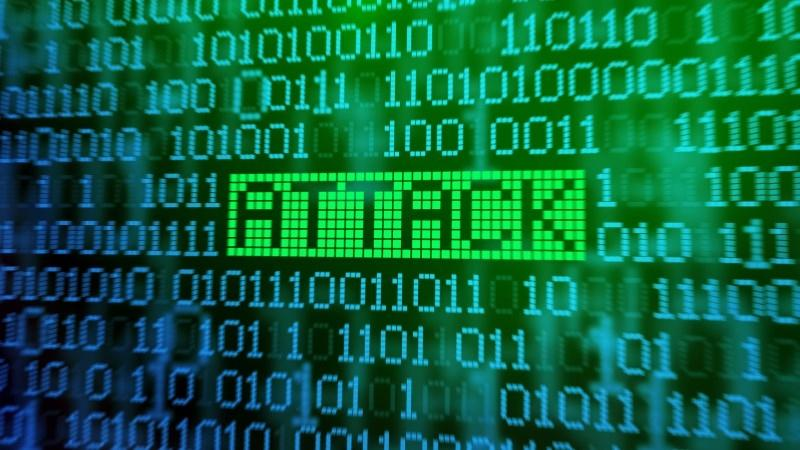
\includegraphics[height=0.8\paperheight, center]{attack}
\end{frame}

\begin{frame}
\frametitle{AVS WINVote (1)}
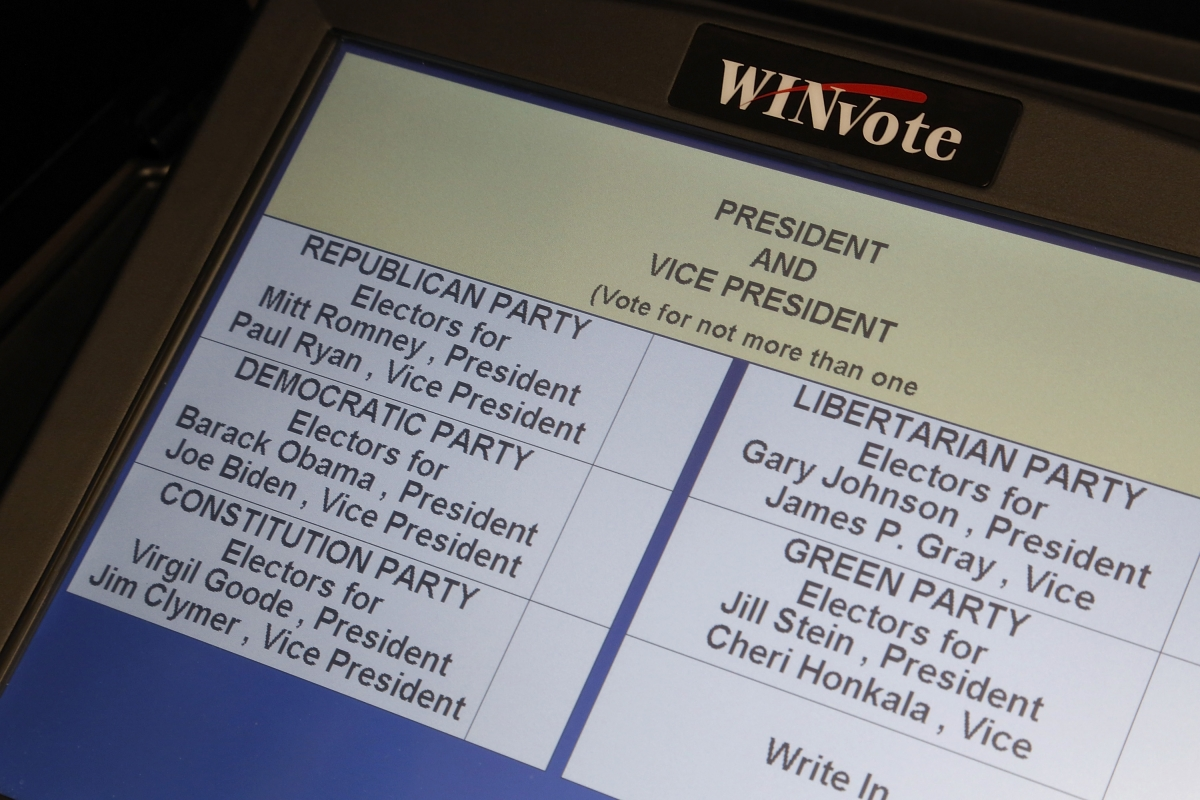
\includegraphics[height=0.7\paperheight, center]{avs-winvote} \\
Urządzenia DRE produkowane przez firmę \textit{Advanced Voting Solutions}. \pause Używane w 3 stanach USA: Pensylwanii, Missisipi i Virginii.
\end{frame}

\begin{frame}
\frametitle{AVS WINVote (2)}
W 2015 roku zlecono kontrolę bezpieczeństwa. Lista znalezionych luk jest imponująco wręcz długa. Oto ona: \pause
\begin{itemize}
\item maszyny połączone były bezprzewodową siecią LAN, zabezpieczoną przestarzałym protokołem WEP; hasło zostało ustawione na ``abcde'', a jego zmiana nie była możliwa, \pause
\item system operacyjny był wersją Windowsa XP, a ostatnia łatka bezpieczeństwa została zainstalowana w 2004, \pause
\item hasło administratora systemu było ustawione na ``admin'', \pause
\item opcja udostępniania plików w sieci była włączona, \pause
\item urządzenie zapisywało pliki w bazie MS Access zabezpieczonej przez krótkie hasło (``shoup''), \pause
\item system nie rejestrował zmian w bazie danych, \pause
\item fizyczne porty nie były w żaden sposób zabezpieczone. 
\end{itemize}
\end{frame}

\begin{frame}
\frametitle{Jak zaatakować wybory? (1)} \pause
\begin{enumerate}
\item Weź laptopa do lokalu wyborczego i usiądź na parkingu. \pause
\item Złam proste hasło WEP. \pause
\item Podłącz się do sieci WiFi. \pause
\item Jeśli zostaniesz poproszony o hasło administratora, wpisz ``admin''. \pause
\item Przez opcję udostępniania plików ściągnij bazę danych z głosami. \pause
\item Za pomocą prostego, darmowego narzędzia złam hasło do bazy danych (``shoup''). \pause
\item Za pomocą Accessa zmieniaj, usuwaj i dodawaj głosy według uznania. \pause
\item Wgraj zmienioną bazę danych z powrotem na serwer. 
\end{enumerate}
\end{frame}

\begin{frame}
\frametitle{Jak zaatakować wybory? (2)}
Po kontroli maszyny utraciły certyfikat. Do wyborów zostały dwa miesiące, a wszystkie urządzenia musiały zostać zastąpione. \pause
\begin{block}{Jeremy Epstein, Freedom To Tinker}
Bottom line is that *if* no Virginia elections were ever hacked (and we have no way of knowing if it happened), it’s because no one with even a modicum of skill tried.
\end{block}
\end{frame}


\begin{frame}
\frametitle{Diebold AccuVote-TS (1)}
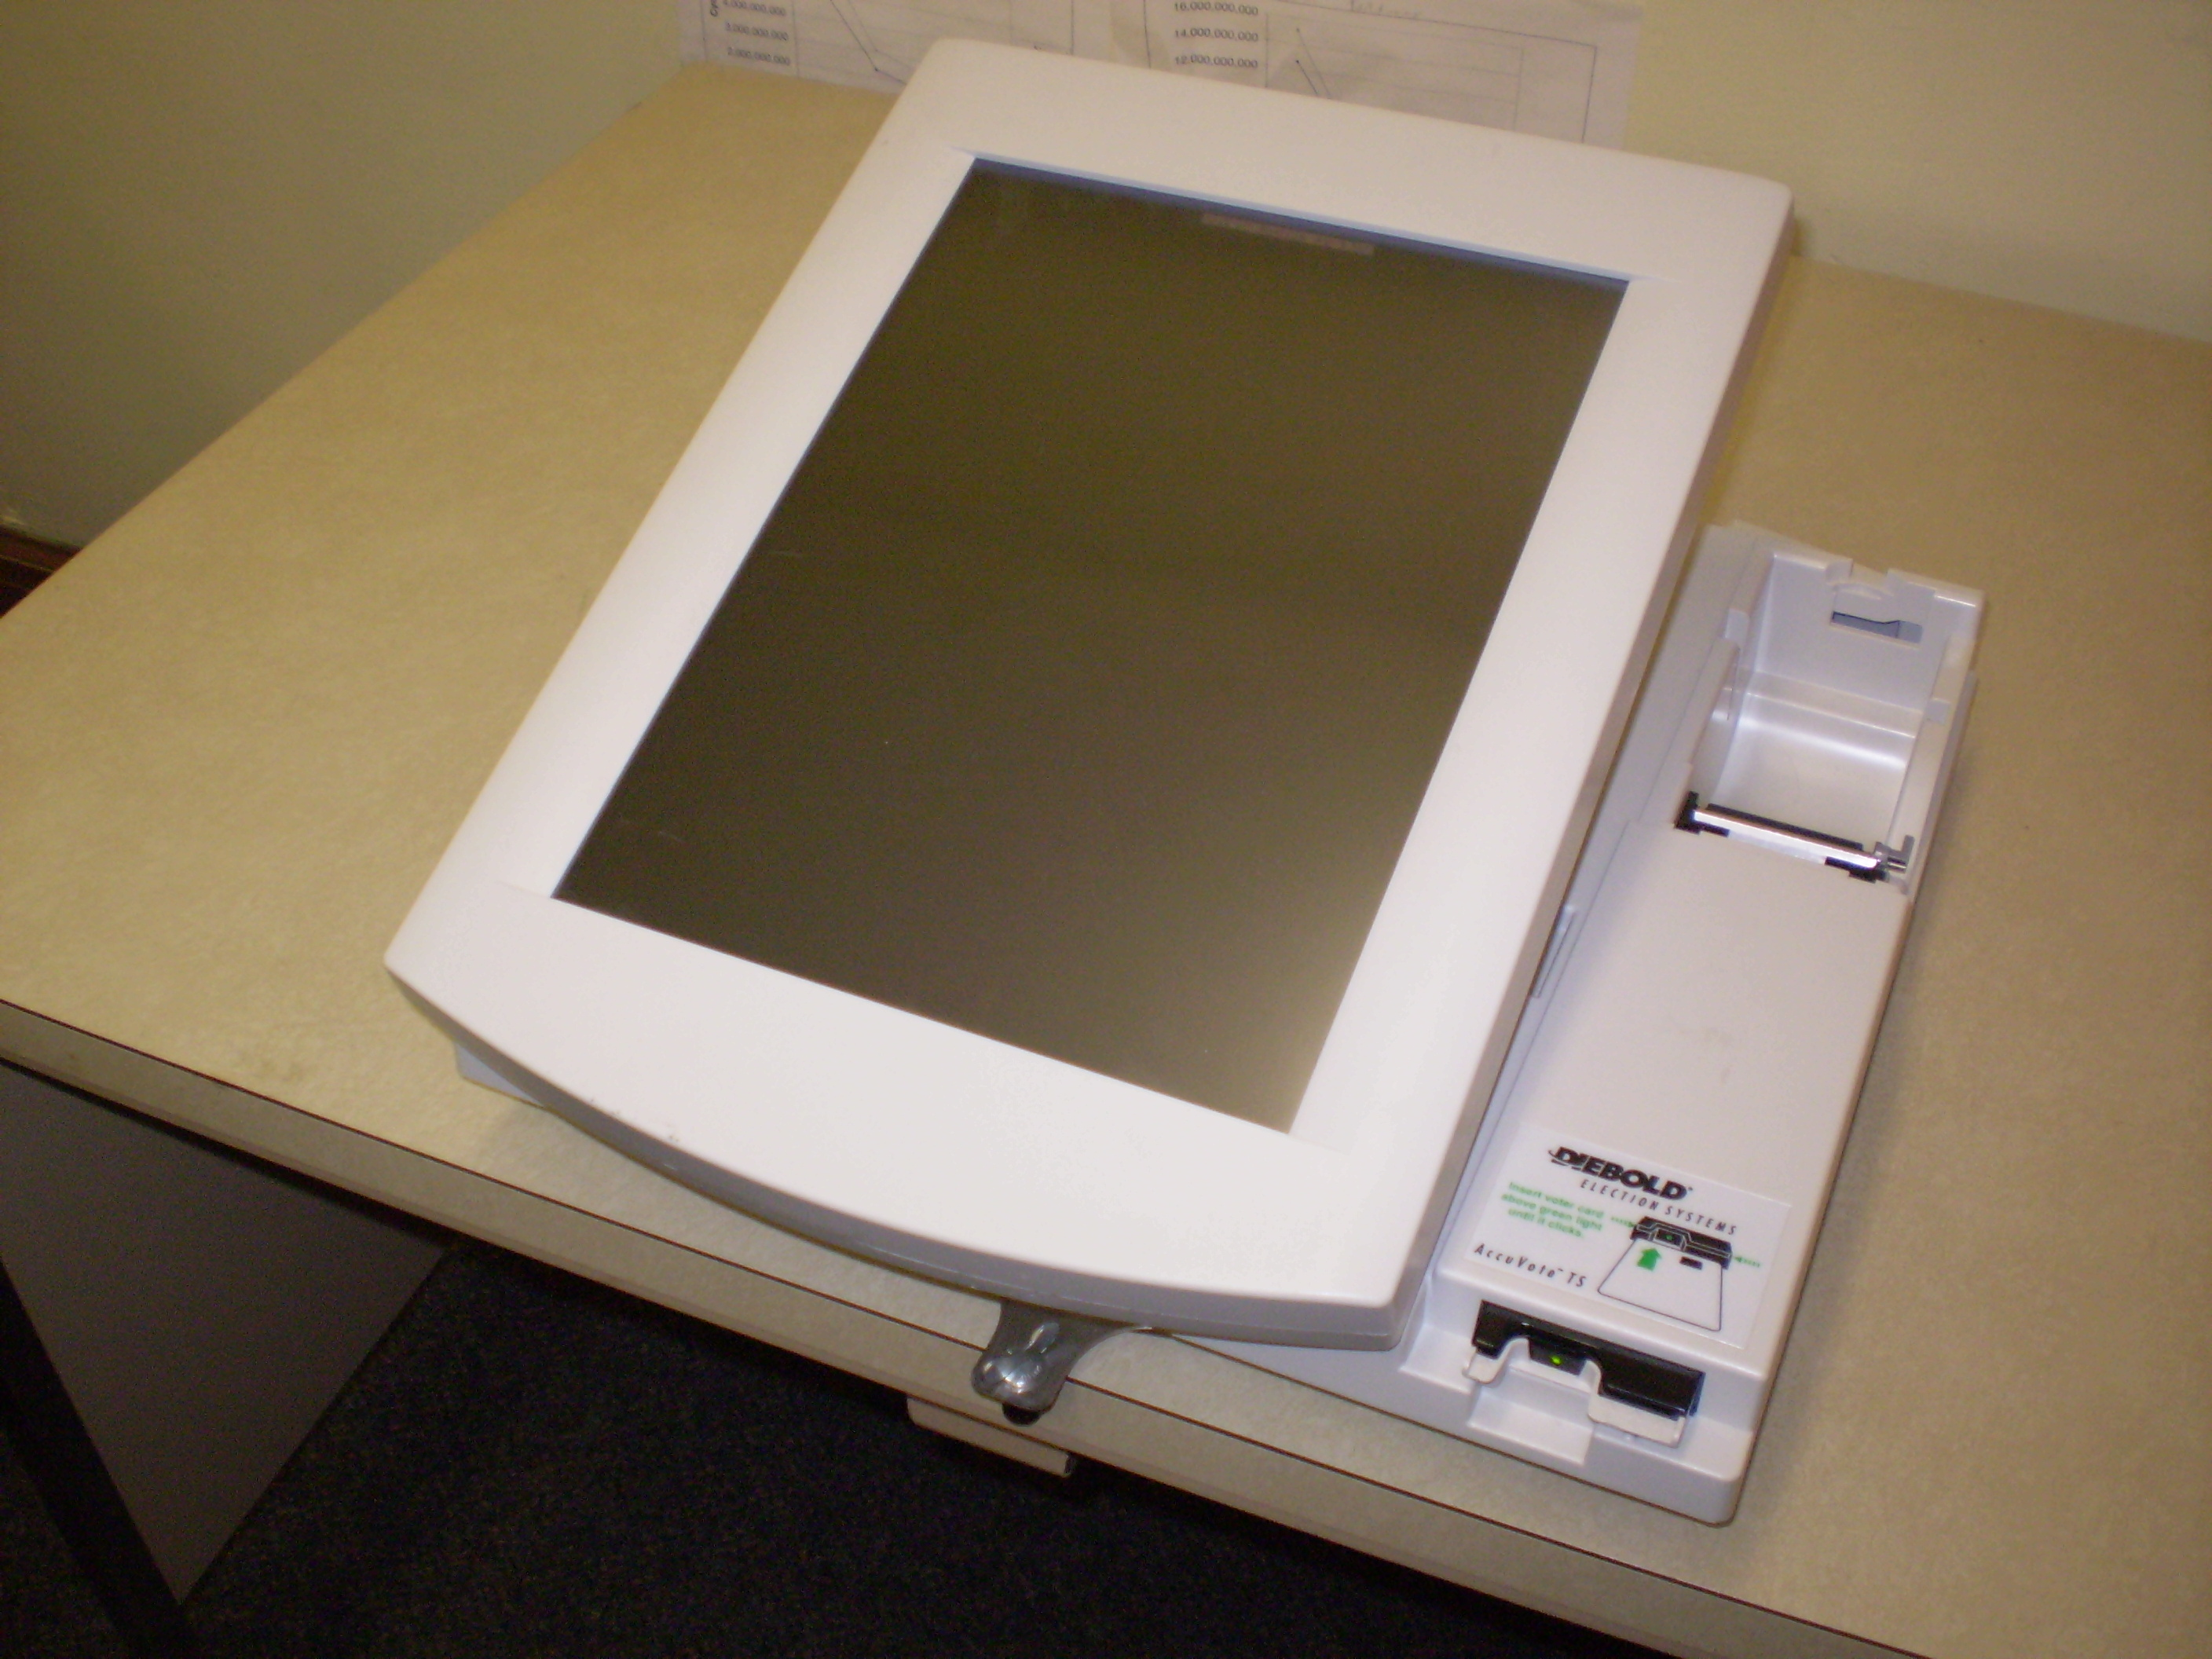
\includegraphics[height=0.6\paperheight, center]{diebold} \\
Rozwiązanie DRE od firmy \textit{Diebold Election Systems} (produkującej DRE dla Brazylii). \pause Kiedyś najpopularniejsze urządzenie DRE w USA. W wyborach w 2006 oddano przy jego pomocy 10\% wszystkich głosów.
\end{frame}

\begin{frame}
\frametitle{Diebold AccuVote-TS (2)}
\begin{itemize}
\item Grupa naukowców z Princeton University dokonała analizy bezpieczeństwa tego systemu. \pause
\item Odkryli, że możliwe było wgranie złośliwego kodu na maszynę. \pause
\item Taki kod mógłby wykradać głosy i zacierać za sobą ślady. \pause
\item Naukowcom udało się stworzyć wirusa instalującego złośliwy kod na innych maszynach (mimo braku połączenia z internetem). \pause
\item Zaatakowanie tej maszyny było trudniejsze niż WINVote'a, ale w razie powodzenia mogło wpłynąć na większą liczbę głosów. 
\end{itemize}
\end{frame}

\begin{frame}
\frametitle{Inne przypadki (e-voting)} \pause
\begin{itemize}
\item W 2007 Sekretarz Stanu Kalifornia zarządziła kontrolę używanych tam systemów DRE. Ekspertyza wykazała podatności wszystkich rozwiązań na wykradanie głosów i złamanie prywatności . Uznano, że błędy są na tyle poważne, że działający w pojedynkę przestępca (niekoniecznie ekspert) mógłby zagrozić bezpieczeństwu wyborów w całym stanie. \pause
\item Okazuje się, że uzyskanie certyfikatu od władz nie gwarantuje bezpieczeństwa. \pause
\item Wykryto podatność komputera wyborczego \textit{Nedap ES3B} podobną do tej znalezionej w AccuVote-TS. Za jego pośrednictwem oddawano w Holandii 90\% głosów. \pause
\item Podobny problem dotyczył rozwiązania stosowanego w Indiach. \pause
\item Nie tylko systemy DRE - udało się też zaatakować urządzenia do skanowania optycznego.
\end{itemize}
\end{frame}

\begin{frame}
\frametitle{Testowanie w Waszyngotnie (1)}
\begin{itemize}
\item W 2010 w Waszyngtonie zdecydowano się stworzyć system do internetowego głosowania dla żołnierzy i ekspatriantów. \pause
\item Na tydzień przed rzeczywistymi wyborami zdecydowano się przeprowadzić wybory próbne. \pause
\item Każdy mógł przetestować zabezpieczenia bez konsekwencji. \pause
\item Kod systemu został opublikowany. Okazało się, że zawierał błędy. \pause
\item Naukowcy odnaleźli lukę, która pozwoliła im przejąć kontrolę nad serwerem.
\end{itemize}
\end{frame}

\begin{frame}
\frametitle{Testowanie w Waszyngotnie (2)}
\begin{itemize}
\item Udało się uzyskać dostęp do kamer monitoringu.\pause
\item Atakujący najpierw wykradli wszystkie hasła.\pause
\item Później zmienili oddane głosy na swoje.\pause
\item Dodali kod, który modyfikował nowe głosy.\pause
\item Dodali backdoor, który pozwalał im podglądać głosy.\pause
\item Wyczyścili wszystkie logi.
\end{itemize}
\end{frame}

\begin{frame}
\frametitle{Testowanie w Waszyngotnie (3)}
\begin{itemize}
\item Atakujący celowo zostawili ślad.\pause
\item Włamanie zostało wykryte dopiero po dwóch dniach.\pause
\item Waszyngton zrezygnował z systemu i zezwolił na przesyłanie głosów pocztą.
\end{itemize}
\end{frame}

\begin{frame}
\frametitle{Jak zaatakować wybory w Estonii?}
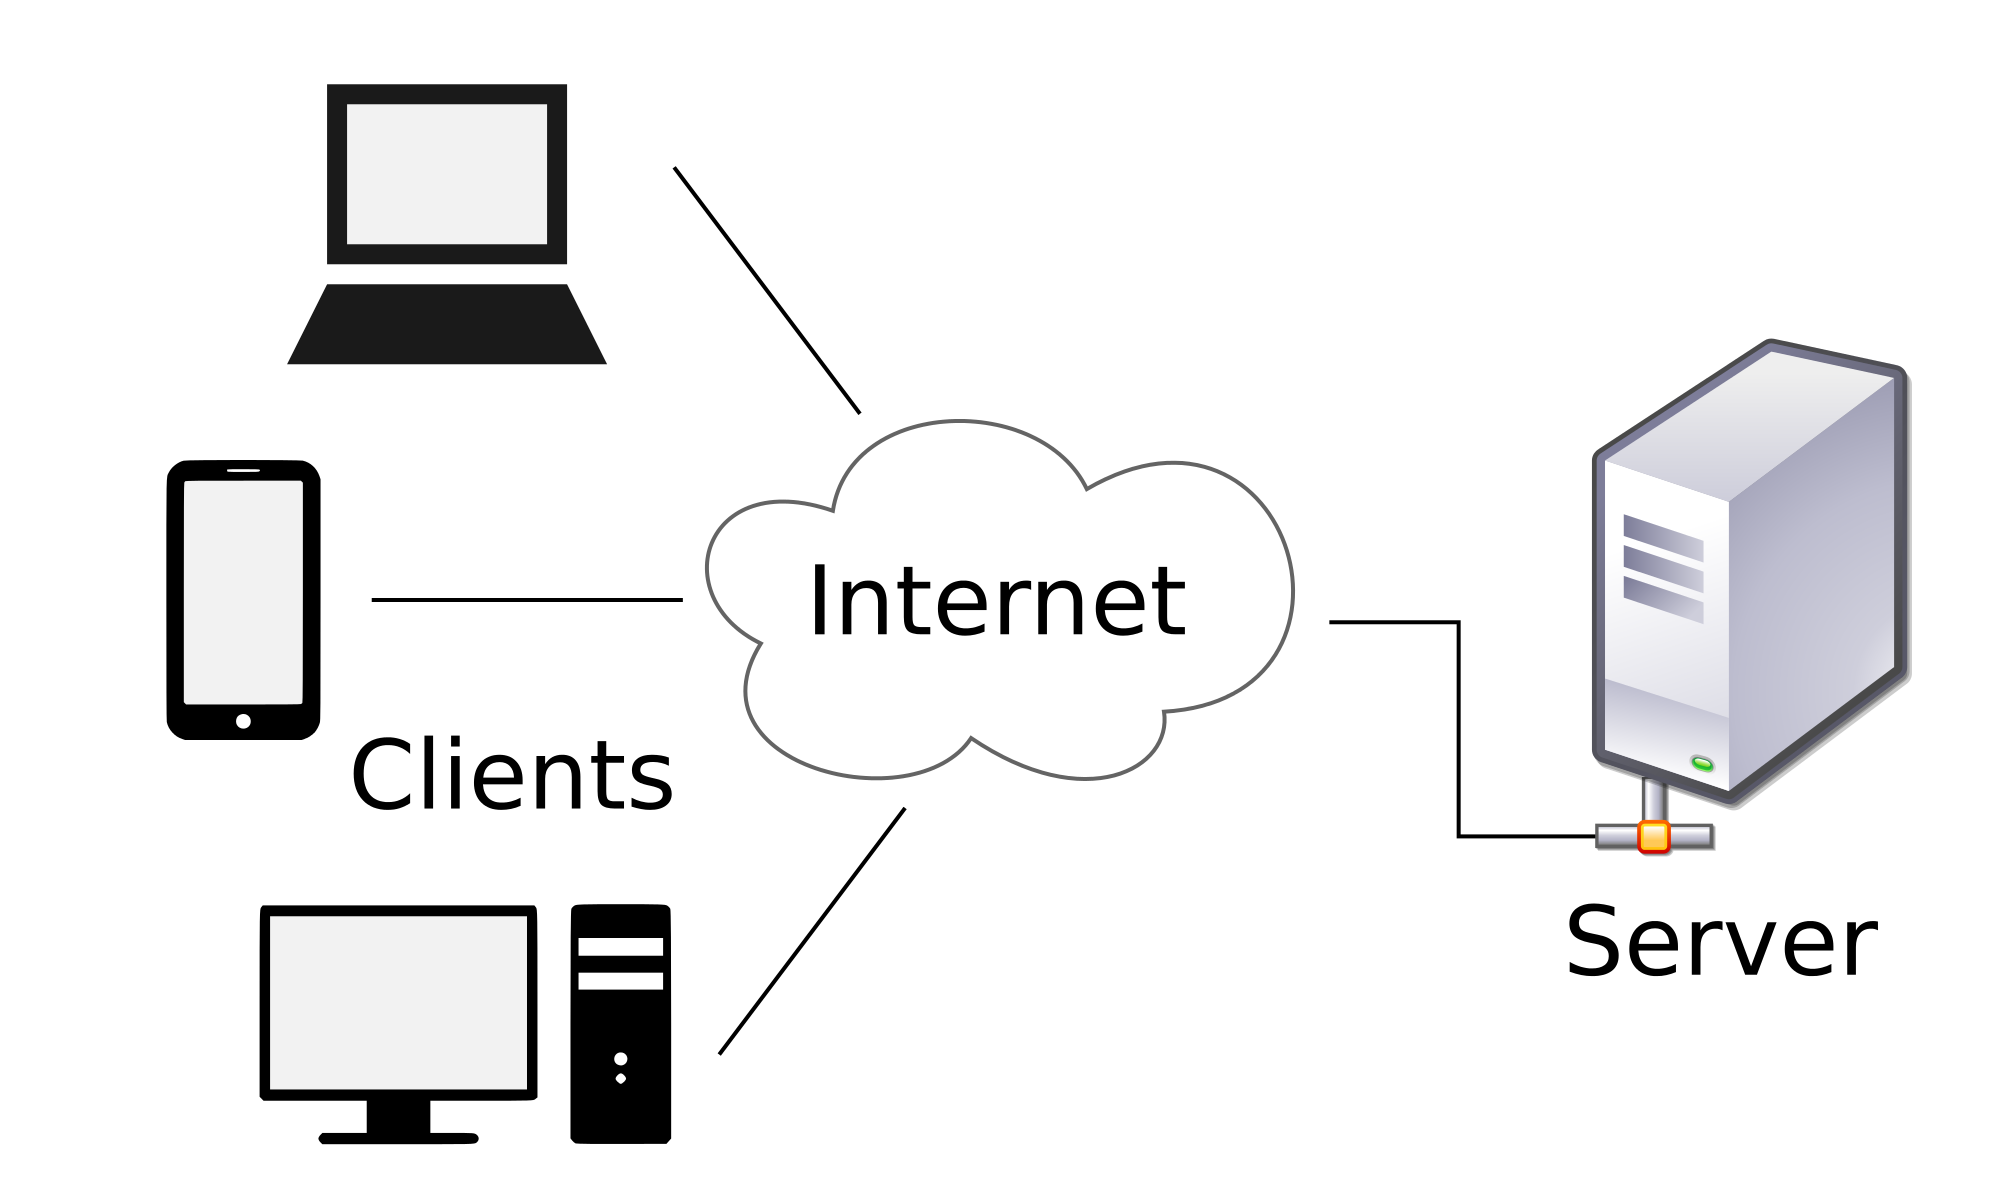
\includegraphics[height=0.8\paperheight, center]{client-server}
\end{frame}

\begin{frame}
\frametitle{Kto mógłby spróbować?}
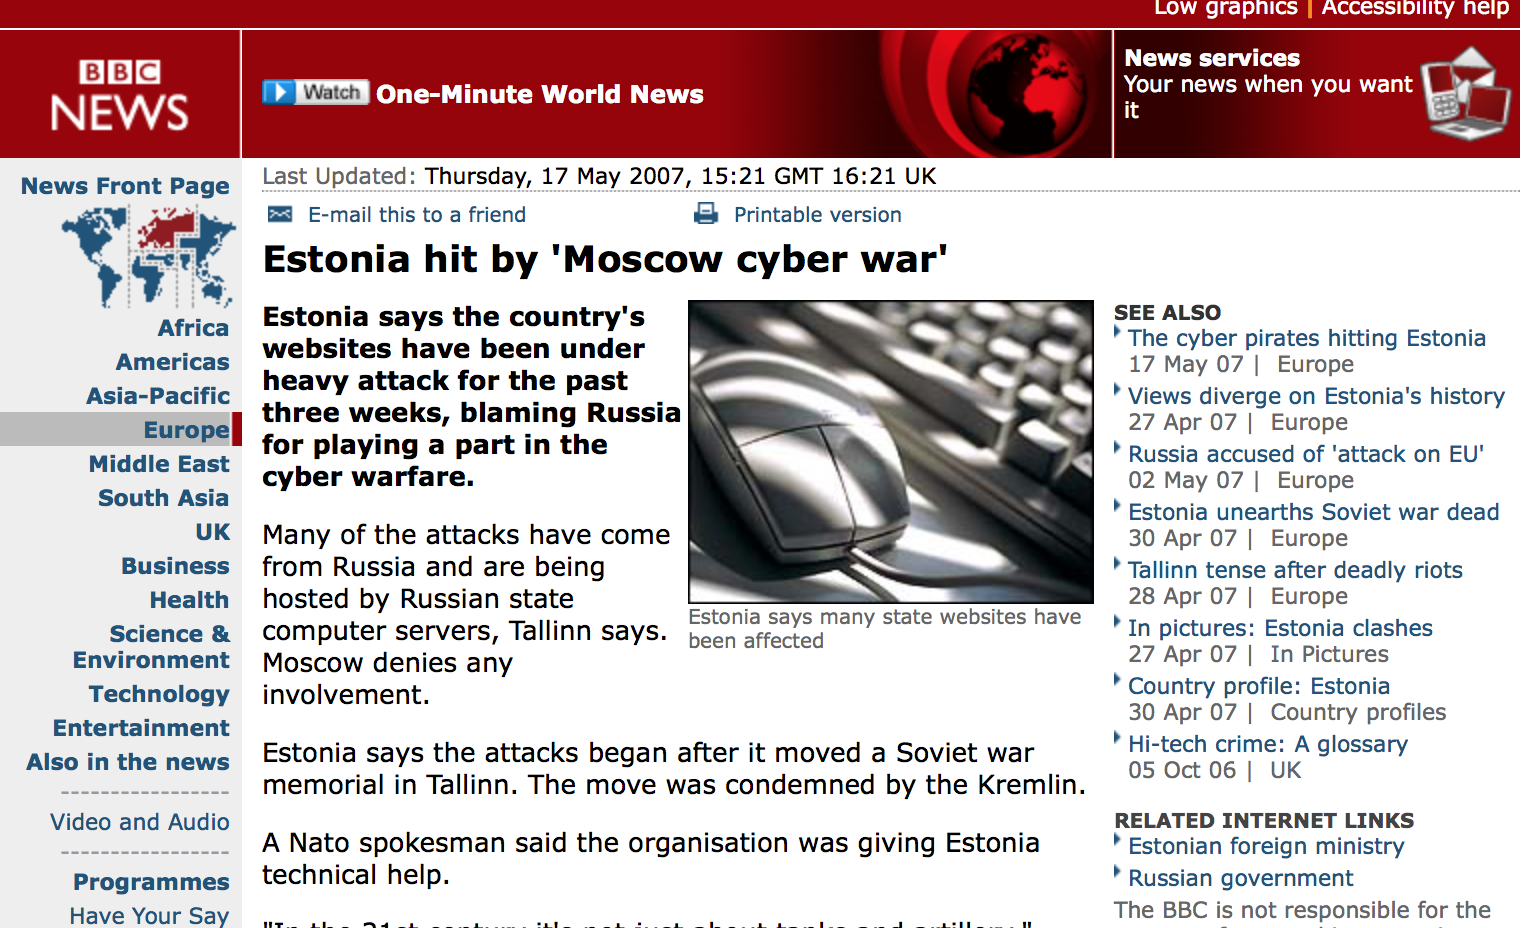
\includegraphics[height=0.8\paperheight, center]{cyberwar}
\end{frame}

\begin{frame}
\frametitle{Atak od strony serwera (1)}
\begin{itemize}
\item Metody zbliżone do ataków na systemy DRE. \pause
\item Atakujący wgrywa złośliwy kod na komputer gromadzący lub zliczający głosy. \pause
\item Trudniejszy i łatwiejszy do wykrycia niż atak na klienta. \pause
\item W efekcie daje kontrolę nad wszystkimi głosami. \pause
\item W Estonii kod serwera jest publiczny.
\end{itemize}
\end{frame}

\begin{frame}
\frametitle{Atak od strony serwera (2)}
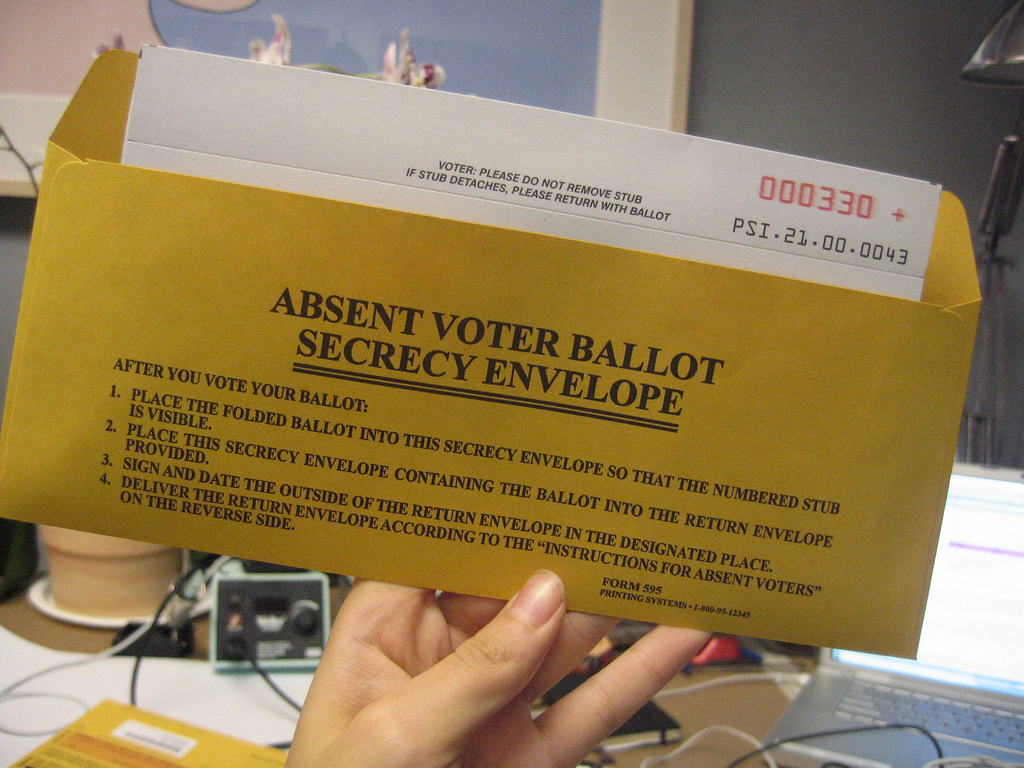
\includegraphics[height=0.8\paperheight, center]{envelope}
\end{frame}

\begin{frame}
\frametitle{Atak od strony serwera (3)}
\begin{itemize}
\item Atakujący musi dostać się do serwera zliczającego głosy. \pause
\item Sam serwer jest dość dobrze zabezpieczony. \pause
\item Ale na czymś przecież go napisano... \pause
\item Okazuje się, że możliwe jest zaatakowanie serwera deweloperskiego. \pause
\item Potem jest już łatwo. \pause
\item Bezpieczeństwo wyborów zależy od bezpieczeństwa operacyjnego. W Estonii nie było najlepiej...
\end{itemize}
\end{frame}

\begin{frame}
\frametitle{Atak od strony klienta (1)}\pause
\begin{itemize}
\item Klient to najsłabsze ogniwo.\pause
\item Według analityków da się napisać wirusa, który bez wiedzy wyborcy zmieni jego głos. Taki wirus mógłby ominąć wszystkie zabezpieczenia estońskiego systemu (e-dowód, PIN i aplikację weryfiukjącą).\pause
\item Atakujące może tak zmienić jeden głos. A co jeśli jest właścicielem botnetu? A co jeśli jest właścicielem wielu botnetów?\pause
\item W Estonii kod klienta jest tajny.\pause
\item Jeden z nich zademonstrował estoński student - Paavo Pihelglas. Zażądał unieważnienia wyborów, ale przegrał przez sądem. Wymiar sprawiedliwości uznał, że skoro on sam, dobrowolnie stowrzył wirusa, to jego prawa nie zostały pogwałcone.
\end{itemize}
\end{frame}

\begin{frame}
\frametitle{Atak od strony klienta (2)}
\begin{itemize}
\item  Atakujący musi zainstalować swojego wirusa na komputerze klienta.\pause
\item Wirus wykrada PIN wyborcy.\pause
\item I zmienia głos bez wiedzy użytkownika.\pause
\item Analitycy zademonstrowali jak ominąć aplikację weryfikacyjną.\pause
\item Jak zainstalować wirusy?
\end{itemize}
\end{frame}

\begin{frame}
\frametitle{Zagrożenia}

\includegraphics[height=0.8\paperheight, center]{danger}
\end{frame}

\begin{frame}
\frametitle{Podstawowe wymagania}\pause
\begin{enumerate}
\item Rzetelność - system musi dokładnie oddać wolę narodu.\pause
\item Anonimowość - każdy głos powinien być całkowicie tajny. Nikt nie może mieć możliwości udowodnienia, że na kogoś głosował.\pause
\item Dostępność - wybory muszą odbyć się w wyznaczonym terminie.\pause
\item Przejrzystość - metoda przeprowadzania wyborów musi być prosta, przejrzysta i zrozumiała. Musi być możliwe obserwowanie całego procesu.\pause
\item Bezpieczeństwo - system musi działać sprawnie nawet w przypadku spisku oraz ataku hakerskiego. Musi istnieć metoda na wykrycie prób ataku i skontrolowanie wyniku.
\end{enumerate}
\end{frame}

\begin{frame}
\frametitle{Bezpieczeństwo narodowe}
\begin{itemize}
\item W praktyce stworzenie takiego systemu jest trudne.\pause
\item Bezpieczeństwa wyborów to bezpieczeństwo narodowe (nie komercyjne).\pause
\item Głosowanie papierowe nie jest idealne, ale im więcej głosów chcemy ukraść, tym trudniejsza jest organizacja ataku. Inaczej jest z głosowaniem elektronicznym.\pause
\item Wystarczy nam system przynajmniej tak bezpieczny, jak głosowanie papierowe.
\end{itemize}
\end{frame}

\begin{frame}
\frametitle{Przejrzystość (e-voting)}\pause
\begin{itemize}
\item DRE przyjmuje głosy i wydaje werdykt.\pause
\item Skąd wyborca ma mieć pewność, że oprogramowanie działa tak, jak zapewnia producent?\pause
\item Jednym z rozwiązań jest opublikowanie kodu źródłowego.\pause
\item Skąd wyborca ma wiedzieć, że kod, który faktycznie działa na maszynie to ten, który został opublikowany?\pause
\item Może zaufać.\pause
\item Albo sprawdzić sumami kontrolnymi.
\end{itemize}
\end{frame}

\begin{frame}
\frametitle{Bezpieczeństwo (e-voting)}
\begin{itemize}
\item DRE są często podatne.\pause
\item Być może atakom dałoby się zapobiec poprzez dalsze zabezpieczenia.\pause
\item Implementacja może być błędna, a rozwiązanie niekompletne.\pause
\item Im więcej zabezpieczeń, tym mniej ludzi ufa systemowi. Im mniej ludzi ufa systemowi, tym mniej ludzi ufa wynikom.\pause
\item Co jeśli ktoś zaatakuje producenta? Używając DRE uzależniamy bezpieczeństwo narodowe od wewnętrznych zabezpieczeń korporacji.
\end{itemize}
\end{frame}

\begin{frame}
\frametitle{Problemy z i-votingiem (1)}\pause
\begin{itemize}
\item Łańcuch komunikacyjny pomiędzy wyborcą, a centralnym serwerem jest długi.\pause
\item Taki system może zaatakować każdy - od samotnego hakera, do agencji wywiadowczej obcego rządu.\pause
\item Atakujący może cały proces przeprowadzić z dowolnego miejsca na świecie.\pause
\item Może nastąpić kilka ataków jednocześnie. \pause
\item Jeden atak może wpłynąć na wynik całych wyborów.\pause
\item Centralny serwer działa podobnie do maszyny DRE, więc jest podatny na te same ataki. Trzeba zatem:\pause
\begin{itemize}
\item zweryfikować oprogramowanie serwera,\pause
\item zabezpieczyć go przed atakiem hakerów,\pause
\item zaufać dostawcy oprogramowania, że jego serwery były bezpieczne\pause
\item dodatkowo: zapewnić, że serwer będzie działa (DDoS)
\end{itemize}
\end{itemize}
\end{frame}

\begin{frame}
\frametitle{Problemy z i-votingiem (2)}
\begin{itemize}
\item Dodatkowy problem: weryfikacja i autoryzacja wyborcy z zachowaniem anonimowości i przejrzystości.\pause
\item Nie można nic certyfikować - za wiele się zmienia. \pause
\item Pozostają ataki na transmisję i klienta.\pause
\item Nad tymi elementami procesu praktycznie nie ma kontroli. \pause
\item Atak na transmisję - przechwytywanie formularzy.\pause
\item Ataki na klienta - wirusy.
\end{itemize}
\end{frame}

\begin{frame}
\frametitle{Kontrola wyniku}\pause
\begin{itemize}
\item Zabezpieczenie jakiegokolwiek oprogramowania przed \textit{wszystkimi} atakami nie jest możliwe.\pause
\item Musi istnieć możliwość ponownego skontrolowania wyniku wyborów i wykrycia próby manipulacji (niezależna od systemu informatycznego).\pause
\item W przypadku głosowania czysto elektronicznego nie jest to możliwe, bo nie ma trwałego śladu po głosach wyborców.
\end{itemize}
\end{frame}

\begin{frame}
\frametitle{Zagrożenie bezpieczeństwa narodowego}
\begin{itemize}
\item Niektóre ataki mogą zostać przeprowadzone przez jedną osobę.\pause
\item Gdyby się powiodły, mogłyby wpłynąć na wynik całych wyborów. \pause
\item W razie wątpliwości niemożliwe byłoby przeprowadzenie kontroli.\pause
\item Problemy z ewentualnym ściganiem atakujących.
\end{itemize}
\end{frame}

\begin{frame}
\frametitle{Lepsze rozwiązania}
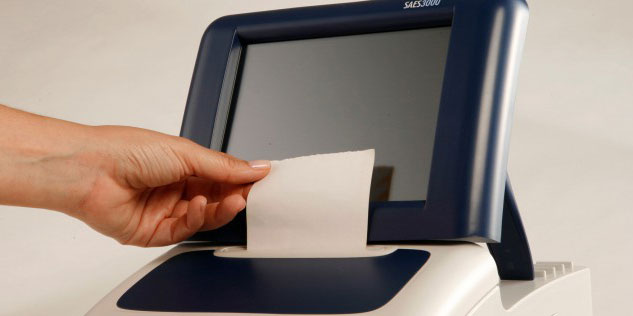
\includegraphics[height=0.8\paperheight, center]{vvpat}
\end{frame}

\begin{frame}
\frametitle{VVPAT}
\begin{itemize}
\item Pozwala wyeliminować najpoważniejszy zarzut - niemożność przeprowadzenia kontroli.\pause
\item Wciąż możemy korzystać z szybkiego przeliczania wyników. \pause
\item Bezpieczeństwo podobne jak przy wyborach tradycyjnych.\pause
\item Wady:\pause
\begin{itemize}
\item W całości zależy od potwierdzania wydruków przez wyborców.\pause
\item Zwiększa koszty i ryzyko awarii. \pause
\end{itemize}
\item Jest wprowadzane w Indiach po wykryciu podatności ich DRE.
\end{itemize}
\end{frame}

\begin{frame}
\frametitle{Prêt à Voter}
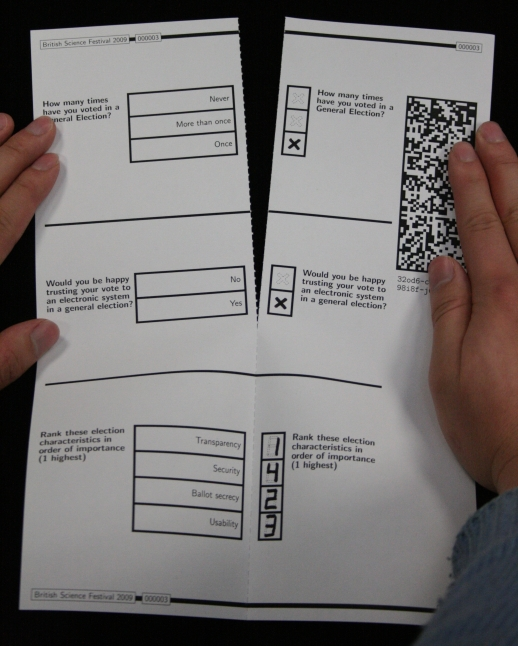
\includegraphics[height=0.8\paperheight, center]{pret}
\end{frame}

\begin{frame}
\frametitle{Dlaczego głosowanie jest tak trudne?}\pause
\begin{block}{Bruce Schneier}
Technology gets in the way of accuracy by adding steps. Each additional step means more potential errors, simply because no technology is perfect.
\end{block}\pause
\begin{itemize}
\item Bezpieczeństwo wyborów należy rozpatrywać w kategorii bezpieczeństwa narodowego.\pause
\item Połączenie wymogów anonimowości, przejrzystości i bezpieczeństwa.\pause
\item Głos każdego wyborcy jest równie istotny.\pause
\item Nikt nie wie, jaki będzie wynik.\pause
\item Szczególny nacisk na bezpieczeństwo - odwrócenie skutków ataku może być trudne.
\end{itemize}
\end{frame}

\begin{frame}
\frametitle{Ostatnie wybory w USA (1)}
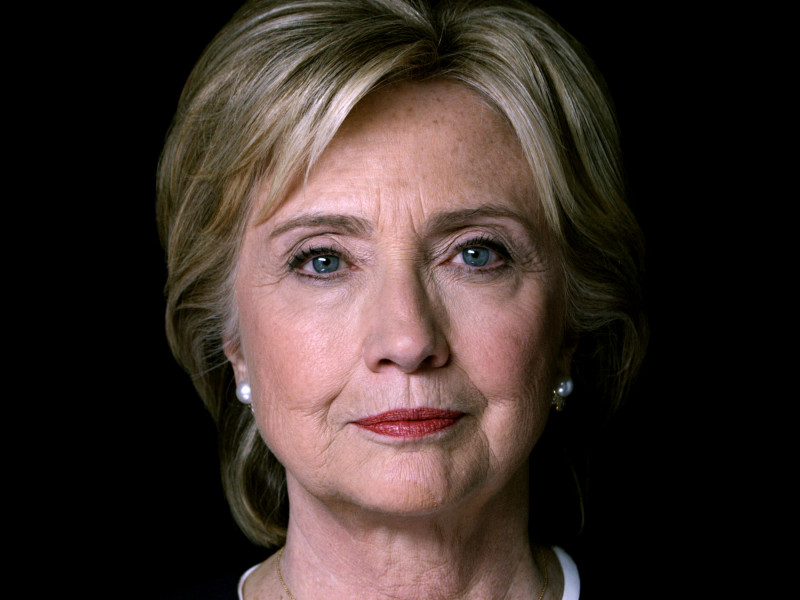
\includegraphics[height=0.8\paperheight, center]{clinton}
\end{frame}

\begin{frame}
\frametitle{Ostatnie wybory w USA (2)} \pause
\begin{itemize}
\item Hillary Clinton otrzymała znacząco mniej głosów w okręgach używających elektroniki niż w tych, gdzie głosuje się papierowo. \pause
\item Dokładnie takiego wyniku oczekiwalibyśmy, gdyby wybory zostały zmanipulowane.\pause
\item Prawdopodobieństwo ataku niskie.\pause
\item Nie ma kto, ani jak tego sprawdzić.\pause
\item Nawet jeśli były zmanipulowane, to nie za bardzo jest jak to odkręcić.\pause
\item Żółta kartka dla elektronicznego głosowania.
\end{itemize}
\begin{block}{Bruce Schneier}
But we only have two years until the next national elections, and it's time to start fixing things if we don't want to be wondering the same things about hackers in 2018. The risks are real: Electronic voting machines that don't use a paper ballot are vulnerable to hacking.
\end{block}
\end{frame}
 
\end{document}